%% Author_tex.tex
%% V1.0
%% 2012/13/12
%% developed by Techset
%%
%% This file describes the coding for rsproca.cls

\documentclass[]{rsos}%%%%where rsos is the template name

%%%% *** Do not adjust lengths that control margins, column widths, etc. ***

%%%%%%%%%%% Defining Enunciations  %%%%%%%%%%%
\newtheorem{theorem}{\bf Theorem}[section]
\newtheorem{condition}{\bf Condition}[section]
\newtheorem{corollary}{\bf Corollary}[section]
%%%%%%%%%%%%%%%%%%%%%%%%%%%%%%%%%%%%%%%%%%%%%%%

\begin{document}

%%%% Article title to be placed here
\title{Information-theoretic measures for non-linear causality detection: \\ application to social media sentiment and cryptocurrency prices}

\author{%%%% Author details
Z. Keskin$^{1,2}$, T.Aste $^{1,3}$}

%%%%%%%%% Insert author address here
\address{$^{1}$Department of Computer Science \& Centre for Blockchain Technologies, University College London, Gower Street, WC1E 6EA, London, United Kingdom.\\
$^{2}$Department of Physics and Astronomy, University College London, Gower Street, WC1E 6EA, London, United Kingdom.
$^3$ UCL Centre for Blockchain Technologies, University College London, London, United Kingdom.}

%%%% Subject entries to be placed here %%%%
\subject{Information Theory, Causality, Computational Statistics, Time Series Analysis}
 
%%%% Keyword entries to be placed here %%%%
\keywords{Granger, Causality, Transfer Entropy, Information Theory, Cryptocurrency}

%%%% Insert corresponding author and its email address}
\corres{Zac Keskin\\
\email{zac.keskin.17@ucl.ac.uk}}

%%%% Abstract text to be placed here %%%%%%%%%%%%
\begin{abstract}
    Information transfer between time series is calculated using the asymmetric information-theoretic measure known as transfer entropy. Geweke's autoregressive formulation of Granger causality is used to compute linear transfer entropy, and Schreiber's general, non-parametric, information-theoretic formulation is used to quantify non-linear transfer entropy. 
    We first validate these measures against synthetic data. Then we apply these measures to detect {\color{blue} statistical causality} between social sentiment and cryptocurrency prices. We validate results by performing permutation tests by shuffling the time series, and calculate the Z-score. We also investigate different approaches for partitioning in nonparametric density estimation which can improve the significance. 
    Using these techniques on sentiment and price data over a 48-month period to August 2018, for four major cryptocurrencies, namely bitcoin (BTC), ripple (XRP), litecoin (LTC) and ethereum (ETH), we detect significant information transfer, on hourly timescales, with greater net information transfer from sentiment to price for XRP and LTC, and instead from price to sentiment for BTC and ETH. We report the scale of non-linear {\color{blue}statistical causality} to be an order of magnitude larger than {\color{blue}the linear case}.
\end{abstract}

%%%%%%%%%%%%%%%%%%%%%%%%%%%

%%%%%%%%%% Insert the texts which can accomdate on firstpage in the tag "fmtext" %%%%%

% \begin{fmtext}
% \section{Insert A head here}
% %%%% Insert A head here

% This demo file is intended to serve as a ``starter file''
% for rsproca journal papers produced under \LaTeX\ using
% rsproca.cls v1.5e.

% \subsection{Insert B head here}
% %%%% Insert B head here
% Subsection text here.

% \subsubsection{Insert C head here}
% %%%% Insert C head here
% Subsubsection text here.

% \section{Equations}

% Sample equations. \cite{1}\cite{1,2} \cite{1,2,3}

% %%% Numbered equation
% \begin{align}\label{1.1}
% \begin{split}
% \frac{\partial u(t,x)}{\partial t} &= Au(t,x) \left(1-\frac{u(t,x)}{K}\right)-B\frac{u(t-\tau,x) w(t,x)}{1+Eu(t-\tau,x)},\\
% \frac{\partial w(t,x)}{\partial t} &=\delta \frac{\partial^2w(t,x)}{\partial x^2}-Cw(t,x)+D\frac{u(t-\tau,x)w(t,x)}{1+Eu(t-\tau,x)},
% \end{split}
% \end{align}

% \begin{align}\label{1.2}
% \begin{split}
% \frac{dU}{dt} &=\alpha U(t)(\gamma -U(t))-\frac{U(t-\tau)W(t)}{1+U(t-\tau)},\\
% \frac{dW}{dt} &=-W(t)+\beta\frac{U(t-\tau)W(t)}{1+U(t-\tau)}.
% \end{split}
% \end{align}

% %%%% Unnumbered equation
% \begin{eqnarray}
% \frac{\partial(F_1,F_2)}{\partial(c,\omega)}_{(c_0,\omega_0)} = \left|
% \begin{array}{ll}
% \frac{\partial F_1}{\partial c} &\frac{\partial F_1}{\partial \omega} \\\noalign{\vskip3pt}
% \frac{\partial F_2}{\partial c}&\frac{\partial F_2}{\partial \omega}
% \end{array}\right|_{(c_0,\omega_0)}\notag\\
% =-4c_0q\omega_0 -4c_0\omega_0p^2 =-4c_0\omega_0(q+p^2)>0.
% \end{eqnarray}
% \end{fmtext}

%%%%%%%%%%%%%%% End of first page %%%%%%%%%%%%%%%%%%%%%

\maketitle


\section{Introduction}

  Causality is a central concept in natural sciences, commonly understood to describe where a process, evolving in time, has some observable effect on a second process. However, the nature of this causative effect is challenging to describe and quantify with precision. There is a long history in determining whether some change truly causes another \cite{hume1738treatise,pearl2009causality}, especially when the relationship is not deterministic, and is observed only in aggregate. In this paper, we consider a statistical form of causality, which can be observed in co-dependent time series where a response in the dependent series is more likely to follow after some change in the driving series. The direction of information transfer is forced by requiring the cause to precede the effect. This concept was conceived first by Wiener in 1956 \cite{Wiener}, and formalised by Granger in 1969 \cite{granger1969investigating} who was subsequently awarded the Nobel memorial prize in economics for his work on the analysis of time series. In simplest terms, the so-called Granger causality describes the extent to which a given series is better able to be predicted by consideration of the information in prior values of another series. If the response in the dependent series scales as a linear multiple of the driving signal, this relationship is described as a linear coupling. If, instead, the response follows some other function of the signal, the relationship is non-linear.

  In modern portfolio theory, investors commonly calculate correlations between asset types to construct portfolios aiming to maximise their return at a given level of risk \cite{markowitz1952portfolio}. In the search for excess returns, quantitative approaches are often exploited to detect predictive signals across time series. In the ideal case,  knowing the movement of one price, the movement of a second can be inferred.  In this paper we explore the effectiveness of two promising techniques for detecting information transfer between time series, applying these to identify causal signals between alternative data and cryptocurrency prices. 

  The concept of an entirely peer-to-peer digital currency managed via a distributed ledger was described and applied by Nakamoto in 2008 \cite{nakamoto2008bitcoin}, who named the currency `Bitcoin'. The proposal and subsequent implementation captured the attention of technologists, economists, libertarians and futurists, and spawned numerous adaptations utilising the blockchain technology \cite{aste2017blockchain}, which have come to be known as cryptocurrencies. Trading in these cryptocurrencies has become widely available even to less sophisticated retail investors, and volumes have grown significantly as interest in the currencies has widened. The crypto market is characterised by high volatility which seems to reflect changes in the attitudes of investors. The usage of cryptocurrencies in the traditional economy remains limited, and it is reasonable to assume that prices are in part driven by speculative dynamics, separate to any utility as a medium of exchange or to any revenue-generating process. Therefore one should expect to observe a larger interplay between sentiment and prices in cryptocurrencies, compared to more fundamental-driven markets such as equities. We discuss existing literature that identifies signals between social sentiment and equity prices, and so hypothesise that investor sentiment on future cryptocurrency prices may be expected to feed into the short-term price movements via speculation, which may be detected using applied information-theoretic techniques. This paper tests this hypothesis. 

  The relationship between social media sentiment and price has been explored in the literature for traditional markets and, more recently, for crypto markets as well, including by an author of this paper. For instance, Bollen et al.  \cite{bollen2011twitter} showed that the mood of Twitter messages can be used as a proxy for market sentiment, and that this can show a linear relationship with price movements in US equities. Zheludev \& Aste \cite{zheludev2014can} also performed sentiment analysis using Natural Language Processing (NLP) on Twitter data, to show sentiment is significantly coupled with price movements for a number of instruments issued by S\&P500 firms. Souza \& Aste  used Twitter messages to model market sentiment, and showed the non-linear predictive relationship may be greater than the linear one \cite{souza2016nonlinear}. 
  
  In the cryptocurrency market specifically, one of the authors of the present paper has recently applied information-theoretic techniques to approaches from network theory to characterise the structure of the market as a complex system \cite{Aste2019}. This provided evidence that the market forms a complex, causally-interrelated network linking prices and sentiments across multiple currencies.

  Within a linear causality framework, hypothesising that cryptocurrency price depends on prior values of both price and market sentiment, a Granger causality test can detect the impact of past values of a variable $X_t$ on future values of another variable $Y_t$ \cite{granger1969investigating}. This can be calculated using a vector auto-regressive (VAR) model, which describes the extent to which including past values of $X$ reduces the sum of squared residuals in the regression of $X$ against $Y$, hence estimating the predictive effect, at each lag $k$, of the social sentiment at $t-k$ on the price at time $t$. 

  The VAR approach performs a regression analysis which is limited to linear associations between variables. To investigate non-linear relations, we can adopt techniques developed in information theory. Many popular information-theoretic measures for comparing distributions, such as mutual information, are symmetric and so can not model a directional information transfer from $X$ to $Y$. Therefore, to generalise Granger causality to the non-linear case, we adopt the measure formalised by Schreiber \cite{schreiber2000measuring}, known as transfer entropy, which is able to capture the size and also the direction of information transfer.

  Transfer entropy arises from the formulation of conditional mutual information; it quantifies the reduction in uncertainty about the dependent time series provided by the past values of the driving signal, conditioning on the past values of the dependent variable itself. This presents a natural way to model statistical causality between variables in multivariate distributions. In the general formulation, transfer entropy is a model-free statistic, able to measure the time-directed transfer of information between stochastic variables, and therefore provides an asymmetric method to measure information transfer. As presented in this paper, transfer entropy appears naturally as a generalisation of Granger causality. In fact it has been shown that, for multivariate normally-distributed statistics, where the relationship is therefore linear, this is indeed the case: Granger causality and transfer entropy are equivalent \cite{barnett2009granger}.

  Though developed relatively recently, information-theoretic methods have been used with success in research across disciplines, to detect information transfer where interventionist approaches are not possible. For example, in neuroscience, Vicente et al. \cite{vicente2011transfer} found transfer entropy to be a superior measure in {\color{blue} detecting Granger causality} in electrophysiological communication than {\color{blue}the auto-regressive formulation}. In climatology, Liang derived from first principles a linear information flow measure, and used this to show that El Ni\~{n}o tends to stabilise the Indian Ocean Dipole \cite{san2014unraveling}. This analysis also detected a causal effect in the other direction; the Indian Ocean Dipole was shown to amplify El Ni\~{n}o oscillations. The technique was used with further success by Stips et al. \cite{stips2016causal} to confirm that recent CO$_2$ emissions show a one-way causality towards global mean temperature anomalies, but that on paleoclimate timescales, this direction is reversed and temperatures drive CO$_2$ levels. Finally, in finance, information transfer was measured between equities indices by Kwon \& Yang, showing that the information transfer was greatest from the US, and greatest towards the APAC region \cite{kwon2008information}. In particular, the S\&P500 was shown to be the strongest driver of other stock indices. In an earlier and somewhat related work, Marschinski \& Kantz   \cite{Marschinski2002} defined and used effective transfer entropy to quantify contagion in financial markets. Similarly, Tungsong et al. \cite{tungsong2018} used transfer entropy to develop upon the previous work by Diebold \& Yilmaz \cite{diebold2009measuring} in quantifying spillover effects between financial markets, generalising the methodology and estimating the time evolution of interconnectedness between financial systems.

 The rest of the paper is organised as follows. In Section \ref{s.background} we provide a brief background on {\color{blue}Granger-Geweke causality} ({\color{blue}the} linear causality measure) and transfer entropy ({\color{blue}the} non-linear causality measure). In Section \ref{s.method} we describe details of the methodology adopted to quantify and validate linear and non-linear {\color{blue}Granger} causality, and the techniques used to generate synthetic series of linear and non-linear causal coupling. Section \ref{s.validation} demonstrates that the methodologies correctly detect {\color{blue}statitical} causality in the linear and non linear case when testing against synthetic data. Results for real data, concerning causality between cryptocurrency price and sentiment, are presented in Section \ref{s.results}. Section \ref{s.conclusions} reports conclusions and perspectives.


\section{Background} \label{s.background}  

  We calculate statistical causality between time series using two different approaches. The first approach involves the application of the Granger-Geweke causality test, which assumes linearity and employs vector auto-regressive techniques to estimate the extent to which knowing the driving time series can improve predictions of the dependent series. The second technique requires an estimation of the transfer entropy, which uses conditional mutual information to quantify the predictability of the dependent series. When predictability is increased by considering the past values of the driving variable, statistical causality is observed.
  
  \subsection{Linear {\color{blue}Granger} Causality}
  
  In the linear approach, we model a time series as autoregressive by expressing its value $Y_t$ at time $t$ as a sum of the contributions over $m$ distinct lagged series, using the linear equation:

  \begin{eqnarray}
    \label{eq:autoregression1}
    Y_t = \sum_{k=1}^m \beta_{k}^{(Y)} \, Y_{t-k} + \epsilon_t ,
  \end{eqnarray}

  where $\beta^{(Y)}_k$ is a general coefficient term and $\epsilon_t$ is the residual. Linear regression estimates the coefficient parameters $\beta^{(Y)}_k$ which minimise the sum of squared residuals. 

  To detect whether the values of some second time series $X$ anticipate the future values of $Y$, we can compare equation \ref{eq:autoregression1}  with: 

  \begin{eqnarray}
    \label{eq:autoregression2}
  Y_t = \sum_{k=1}^m \beta_{k}^{\prime(Y)} \, Y_{t-k}  \; + 
        \sum_{k=1}^m \beta_{k}^{\prime(X)} \, X_{t-k} 
  + \epsilon^{\prime}_t \;.
  \end{eqnarray}

We describe the distribution $Y$ as being Granger-caused by $X$ if the residual in the second regression is significantly smaller than the residual in the first. When this holds, then there must be some information transfer from $X$ to $Y$. Following Geweke \cite{geweke1984measures}, we can represent the information transfer by:

  \begin{eqnarray}
    \label{eq:geweke_measure}
    \operatorname{TE}_{X\rightarrow Y} = \frac12\log \left(
      \frac{\operatorname{var}(\epsilon_t)}
          {\operatorname{var}(\epsilon^{\prime}_t)}
  \right) ,
  \end{eqnarray}

    where we adopt the transfer entropy notation (TE), following the result from Barnett et al. \cite{barnett2009granger} showing Granger causality to be equivalent to transfer entropy for multivariate normal distributions.

  \subsection{Non-Linear {\color{blue}Granger} Causality}

  To detect non-linear {\color{blue}Granger} causality, we apply an information-theoretic approach. Equation \ref{eq:geweke_measure} measures the extent to which the additional information in the lagged variable reduces the variance in the model residuals. Transfer entropy extends this concept by considering the uncertainty, instead of the variance. Adopting Shannon's measure of information \cite{shannon1948}, we can express the uncertainty associated with the continuous random variable $X$ by:

  \begin{eqnarray}
    \label{eq:entropy}
    H(X) = - \int_{-\infty}^{+\infty}  { p(x) \log{p(x)}  } dx,
  \end{eqnarray}
where $p(x)$ is the probability density function.   
$H(x)$ is termed the differential entropy, and it quantifies the uncertainty on the continuous variable $X$. It is an extension of the Shannon entropy for continuous variables. 
In this definition there is an arbitrary additive constant that takes into account the scale factor for the variable $x$, which in this paper we set to zero.
This arbitrary sale factor is a fundamental problem in the definition of Shannon entropy for continuous variables. 
%Indeed, the probability density function $p(x)$ depends on the scale of $x$ and the term $\log p(x)$ should have the probability density function $p(x)$ divided by a scale factor, which in turns introduces the additive constant. 
%In quantum mechanics this problem was solved introducing the Plank length as universal scale factor. 
%In general, outside physical systems, this scale factor rests arbitrary.
However, in the calculation of mutual information and  transfer entropy, these constant factors cancel out, and results are independent of scale.
For discrete variables, where the integral becomes a sum, the constant is equal to zero. Using a logarithm of base 2, the entropy value quantifies the minimum number of bits necessary to encode the signal. 

 Shannon entropy can be directly extended to the multivariate case, defining the joint entropy of two variables $H(X,Y)$ using the joint probability density function $p(x,y)$ in equation \ref{eq:entropy}. Shannon entropy can also be conditioned on a second variable to give the conditional entropy:

  \begin{eqnarray}
    \label{eq:conditional_entropy_2D}
    H(Y | X) = H(X,Y) - H(X) ,
  \end{eqnarray}
Which is the uncertainty on variable $Y$ residual from taking in account all information on variable $X$. 

  %Where two random variables share information, the mutual information is given by:
 The information shared between two variables $X$ and $Y$ is the mutual information:
  \begin{eqnarray}
    \label{eq:mutual_information}
    I(X;Y) = H(Y) - H(Y | X) .
  \end{eqnarray}
 
 Similarly, the entropy of $Y$ conditioned on two variables is:

  \begin{eqnarray}
    \label{eq:conditional_entropy_3D}
    H(Y | X, Z) = H(X,Y,Z) - H(X, Z) ,
  \end{eqnarray}
  
  and the conditional mutual information is therefore:

  \begin{eqnarray}
    \label{eq:conditional_mutual_information}
    I(X;Y|Z) = H(Y|Z) - H(Y | X, Z) .
  \end{eqnarray}

  Now, for each lag $k$, we can describe the information transfer from $X_{t-k}$ to $Y_t$ in terms of the following conditional mutual information:

  \begin{eqnarray}
      \label{eq:TE}
      \operatorname{TE}^{(k)}_{\textbf{}X \rightarrow Y} = I(Y_t ;Y_{t-k} | X_{t-k} ) = H(Y_t | Y_{t-k}) \; - \;  H(Y_t | Y_{t-k}, X_{t-k} ) \;.
  \end{eqnarray}
 This is the reduction of uncertainty in $Y$ when considering the past values of both $Y$ and $X$, compared with considering the past values of $Y$ alone. 

  Considering equations \ref{eq:conditional_entropy_2D} and \ref{eq:conditional_entropy_3D}, we can therefore represent the transfer entropy for a single lag $k$ (equation \ref{eq:TE}), in terms of four separate joint entropy terms. Following equation \ref{eq:entropy}, these may be estimated from the data using a nonparametric  estimation of the probability density functions. For multivariate normal statistics, equations \ref{eq:TE} and \ref{eq:geweke_measure} coincide \cite{barnett2009granger}.


\section{Methods} \label{s.method}

  We calculate linear transfer entropy using ordinary least squares regression, by comparing the variance of the residuals in the joint vector space $ \{Y_t, Y_{t-k}, X_{t-k} \} $ against those in the independent vector space $ \{Y_t, Y_{t-k}\}$, following equation \ref{eq:geweke_measure}. 
  
  To detect non-linear transfer entropy, we perform nonparametric estimation of the probability density functions to calculate the joint entropy terms in equations \ref{eq:conditional_entropy_2D} and \ref{eq:conditional_entropy_3D}. The density is estimated using a multidimensional histogram approach. Histograms have been shown to be effective in estimating entropy, \cite{boba2015efficient}, \cite{Marschinski2002}, but there is a trade-off between bias and variance when partitioning the sample space. The choice of bins impacts the value of the calculated transfer entropy; too fine a partition introduces bias under finite sample size. In this paper we partition the sample space using marginal equi-quantisation, which treats each dimension independently in generating quantile bins such that each marginal bin contains roughly equal numbers of data points \cite{hlavavckova2007causality}. These are used to construct multi-dimensional histograms for estimating the probability distribution. 
Interestingly, to compute relative entropy measures such as mutual information or transfer entropy with a histogram approach, it is sufficient to compute the relative frequencies in each bin, even when bins have non-equal sizes. A note in the Appendix explains why.
  
  The equi-quantisation method has been used previously for the calculation of transfer entropy \cite{hlavavckova2007causality} \cite{darbellay1999estimation}, \cite{Marschinski2002} and it has been shown that it can improve the performance under small sample sizes, by presenting a more precise representation of asymmetric or non-smooth distributions. We observe that using marginal quantile bins can be more robust to varying coarseness than equal-sized bins, as large gradients in the probability distribution function can be captured more closely without the introduction of additional information through refining the partition. 
   

  In estimating Shannon entropy, the coarseness of the partition directly impacts the numerical value, with finely-partitioned histograms returning larger entropy values over the same data, since more information is introduced. This effect should cancel out in the calculation of transfer entropy, however we observe instead that more bins generally results in larger transfer entropies for the same data, which amplifies both signal and noise. We therefore adopt a parsimonious approach in this paper, using a small number of bins compatible with a sufficient resolution, to capture the information transfer. 
  We tested granular partitions using between 3 to 8 bins per dimension, finding comparable results in each case. We report the results using histograms of 6 bins per dimension, a partition size which leads to good and meaningful results for each of the currencies analysed.

  
  It is a feature of the nonparametric estimation of entropy that the absolute scale of the transfer entropy measure has only limited meaning. To detect causality, a relative position must be considered. A simple technique proposed by Marschinski \& Kantz \cite{Marschinski2002} is the Effective Transfer Entropy (ETE), derived by subtracting from the observed transfer entropy an average transfer entropy figure calculated over independently-shuffled time series, which destroys the temporal order and hence any causality.

  We adopt a shuffling approach producing 100 null-hypothesis transfer entropy values from independently shuffled time-series over the same domain, containing no causality. By calculating the mean and standard deviation of the shuffled transfer entropy figures, we estimate the significance of a causal result as the distance between the result and the average shuffled result, standardising by the shuffled standard deviation:
  
  \begin{eqnarray}
    \label{eq:Z-score}
    Z := \frac{\operatorname{TE} - \bar{\operatorname{TE}}_{\operatorname{shuffle}}}
              {\sigma_{\operatorname{shuffle}}} ,
  \end{eqnarray}
  
  where $\operatorname{TE}$ is the transfer entropy of the temporally-ordered sample, $\bar{\operatorname{TE}}_{\operatorname{shuffle}}$ is the average transfer entropy over all shuffled realisations and $\sigma_{\operatorname{shufle}} $ is the standard deviation of the sample of shuffled realisations.
  
  This quantity corresponds to the degree to which the result lies in the right tail of the distribution of the zero-causality shuffled samples, and hence how unlikely the result is due to chance. Therefore the Z-score figure represents the significance of the excess transfer entropy in the un-shuffled case. We compute the Z-score in Eq.\ref{eq:Z-score} for both linear and non-linear results.


  To justify the usage of these techniques in detecting causal relationships in practice, we first validate the methodology using coupled time series of predefined causative relationships. 


  \subsection{Synthetic Geometric Brownian Motion}\label{s.LinearSignal}
  We validate the approach by generating synthetic data following a directionally coupled random walk. First, we generate a driving series, following a discrete Geometric Brownian Motion (GBM):

  \begin{eqnarray}
      \label{eq:GBM}
      X_{t+1} = (1+\mu) X_t + \sigma X_t \; \eta_t ,
  \end{eqnarray}

  where $\eta_t$ is a normally distributed random noise  $\eta_t \sim \mathcal{N}(0,1)$, and $\mu$ and $\sigma$ are respectively drift and diffusion coefficients. Then we produce a second series $Y_t$, which augments a linear dependence on the driving series $X$ with second linear dependence on an independent GBM process $X^{\prime}$. The dependence in both cases is defined at a predetermined lag length $L$, and the strength of these dependencies is determined by some coupling constant $\alpha$, such that with $\alpha=0$, $Y_{t} \equiv X^{\prime}_{t-L}$ i.e. $Y$ is wholly independent of $X$, and in the limiting case $\alpha=1$, $Y$ precisely follows the driving series $X$.

  \begin{eqnarray}
    \label{eq:coupled_random_walk}
    Y_{t} =  \alpha X_{t-L} + (1-\alpha) X^{\prime}_{t-L} .
  \end{eqnarray}

  

  \subsection{Synthetic Coupled Logistic Map}\label{s.NonLinearSignal}
  We generate non-linear coupled time series using a coupled logistic map. This system can be represented in terms of two stationary difference equations; the independent series is defined by the difference equation given by the general update function $f(X)$:

  \begin{eqnarray}
    f(X_t) = X_{t+1} = rX_t(1-X_t)    
    \label{eq:f(x)}
  \end{eqnarray}

  where $X_t$ is the value of $X$ at time $t$, and $r$ is a parameter which in fact defines the dynamical state of the system. {\color{black}Following Hahs \& Pethel \cite{hahs2011distinguishing}, we take $r=4$ so the function evolves chaotically.} We then introduce a second map, which is dependent on the first, taking the form:

  \begin{eqnarray}
    Y_{t} = (1-\alpha) rY_{t-L}(1-Y_{t-L})  + \alpha g(X_{t-L})   
    \label{eq:coupled_map}
  \end{eqnarray}

  where $ \alpha \in [0,1]$ is the cross-similarity, or coupling strength, and $g(x)$ is a coupling function which may be chosen to produce different dynamic effects. In this case only $L=1$ can be used. We follow the choice of Boba et al. \cite{boba2015efficient} and Hahs \& Pethel \cite{hahs2011distinguishing} for the coupling function:

  \begin{eqnarray}
    g(X_t) = (1-\epsilon) f(X_t) + \epsilon f(f(X_t)) 
    \label{eq:g(x)}
  \end{eqnarray}


 where $\epsilon \in [0,1]$ represents the coupling strength, describing the extent to which $Y_{t+1}$ depends on $f(f(X_t))$. It should be noted that the logistic map, in contrast to geometric Brownian motion, is a deterministic, albeit chaotic system, and that therefore $f(f(X_t))$ is equivalent to $X_{t+2}$. {\color{black} The extent of this anticipatory effect is driven by the selection of the $\epsilon$ parameter. We follow Hahs \& Pethel in selecting $\epsilon=0.4$. Indeed, as $\alpha$ increases, with large $\epsilon$, the direction of information transfer is less clear, as $Y_t$ contains more information about the future values of $X$. }



\section{Validation with Synthetic Data} \label{s.validation}

  In order to validate the autoregressive and information-theoretic approaches to detecting causality, we apply these to the calculation of transfer entropy for synthetic data generated by both linear and non-linear coupled time series, of increasing coupling strength. 
  The computations are performed over the relative returns of the synthetic signals generated as described in sections \ref{s.method}\ref{s.LinearSignal} and \ref{s.method}\ref{s.NonLinearSignal}. 
  It is important to note that many areas for which such statistical studies are important are constrained by limited available data. Therefore, for a technique of causal inference to be useful, it must perform even with small sample sizes. In Section \ref{s.results} we apply both classical and information-theoretic methodologies to financial data with sample sizes of the order of $10^4$, and so we first evaluate the performance using synthetic time series of $15,000$ observations, with known causal coupling, before confirming that the technique can detect the same causal coupling with as few as $500$ samples. The results of this evaluation for increasing signal strength, using sample sizes of $500$, $1000$, $2500$, $10,000$ and $100,000$, are presented in Table {\color{blue}2} in the appendix.


  \subsection{Linear Process Causality Validation} 

  We calculate the directional information transfer from the driving series to the dependent series, and in the reverse direction, using both autoregressive and information-theoretic approaches for the linearly-coupled system of GBM walks defined by equations \ref{eq:GBM} and \ref{eq:coupled_random_walk}. Parameters of the independent time series $\mu$ and $\sigma $ are generated independently for each realisation and are distributed normally with $\mathbb{E} [\mu]=0.1$ and $\mathbb{E} [\sigma]=0.025$, and standard deviations of $0.1$ and $0.01$ respectively. Parameters of the endogenous series are also distributed normally around $\mathbb{E} [\mu^{\prime}]=0.1$ and $\mathbb{E} [\sigma^{\prime}]=0.025$, with standard deviations of $0.1$ and $0.01$. Figure \ref{fig:GBM_confirmation} shows the results for coupling strengths from $\alpha = 0.0$ to $\alpha = 0.5$. For each coupling strength, a data set is simulated over 15,000 time steps. Both techniques are applied to each data set to calculate the information transfer, in both directions, with the results from $X \rightarrow Y$ and from $Y \rightarrow X$ plotted on separate axes. 

  In the information-theoretic approach we calculate transfer entropy using histograms with quantile binning of 6 classes per dimension. We generate multiple synthetic coupled random walks, calculating transfer entropy and Z-scores for each realisation, and reporting the mean values. Quantile bins are generated independently for each realisation. We validate causality using the significance testing approach described in Section \ref{s.method}.

  As can be observed from Fig.\ref{fig:GBM_confirmation}, the qualitative correspondence between both methods is clearly visible, and quantitatively the results are similar. Additionally, the one-way direction of information transfer is accurately detected, with large transfer entropy and Z-scores observed in the direction of $X \rightarrow Y$, and approximately-zero values in the opposite direction.


  %\begin{figure*}[!htb]
    
  %\end{figure*}

 
  \subsection{Non-Linear Process Causality Validation}

  We calculate the directional information transfer from the driving series to the dependent series, and in the reverse direction, using both autoregressive and information-theoretic approaches for the non-linear coupled logistic map system from equations \ref{eq:f(x)}, \ref{eq:coupled_map} and \ref{eq:g(x)}.  

  In the information-theoretic approach we calculate transfer entropy again using histograms with quantile binning of 6 classes per dimension, generating bins independently for each realisation.
  
  %\clearpage

  Figure \ref{fig:CLM_confirmation} shows the mean transfer entropy results for 15,000 synthetic data points. We observe that, for this system, the linear method is incapable of detecting the causal relationship; it finds some significant information transfer (at a near-zero level, which we interpret as the linear component), but fails to represent the expected exposure–response relationship and does not correctly identify the expected anticipatory signal in the reverse direction. The information-theoretic method, by contrast, produces results which better represent the increasing coupling strength relationship, and direction of causality in the system. The technique also detects causality from $Y$ to $X$, for large values of $\alpha$. This effect was also observed by Liang and Hahs \& Pethel, and corresponds to the anticipatory nature of the coupling. Specifically the coupling function $g(x)$ involves repeated application of the update function $f(x)$ from equation \ref{eq:f(x)}, from which it can be seen that $f(f(X_t))$ is equivalent to $X_{t+2}$ so, for large $\alpha$, $Y_t$ will contain increasing amounts of the future information of $X_t$. In fact, at large coupling strengths approaching $\alpha=1$, the observed transfer entropy from $X$ to $Y$ begins to decrease, as more information exists in $Y$ about its future evolution.

  The results of these validation experiments suggest that the information-theoretic approach is superior in detecting causal signals, being model-free and so able to detect relationships of more complex, non-linear modes.

  \begin{figure*}[!htb]
    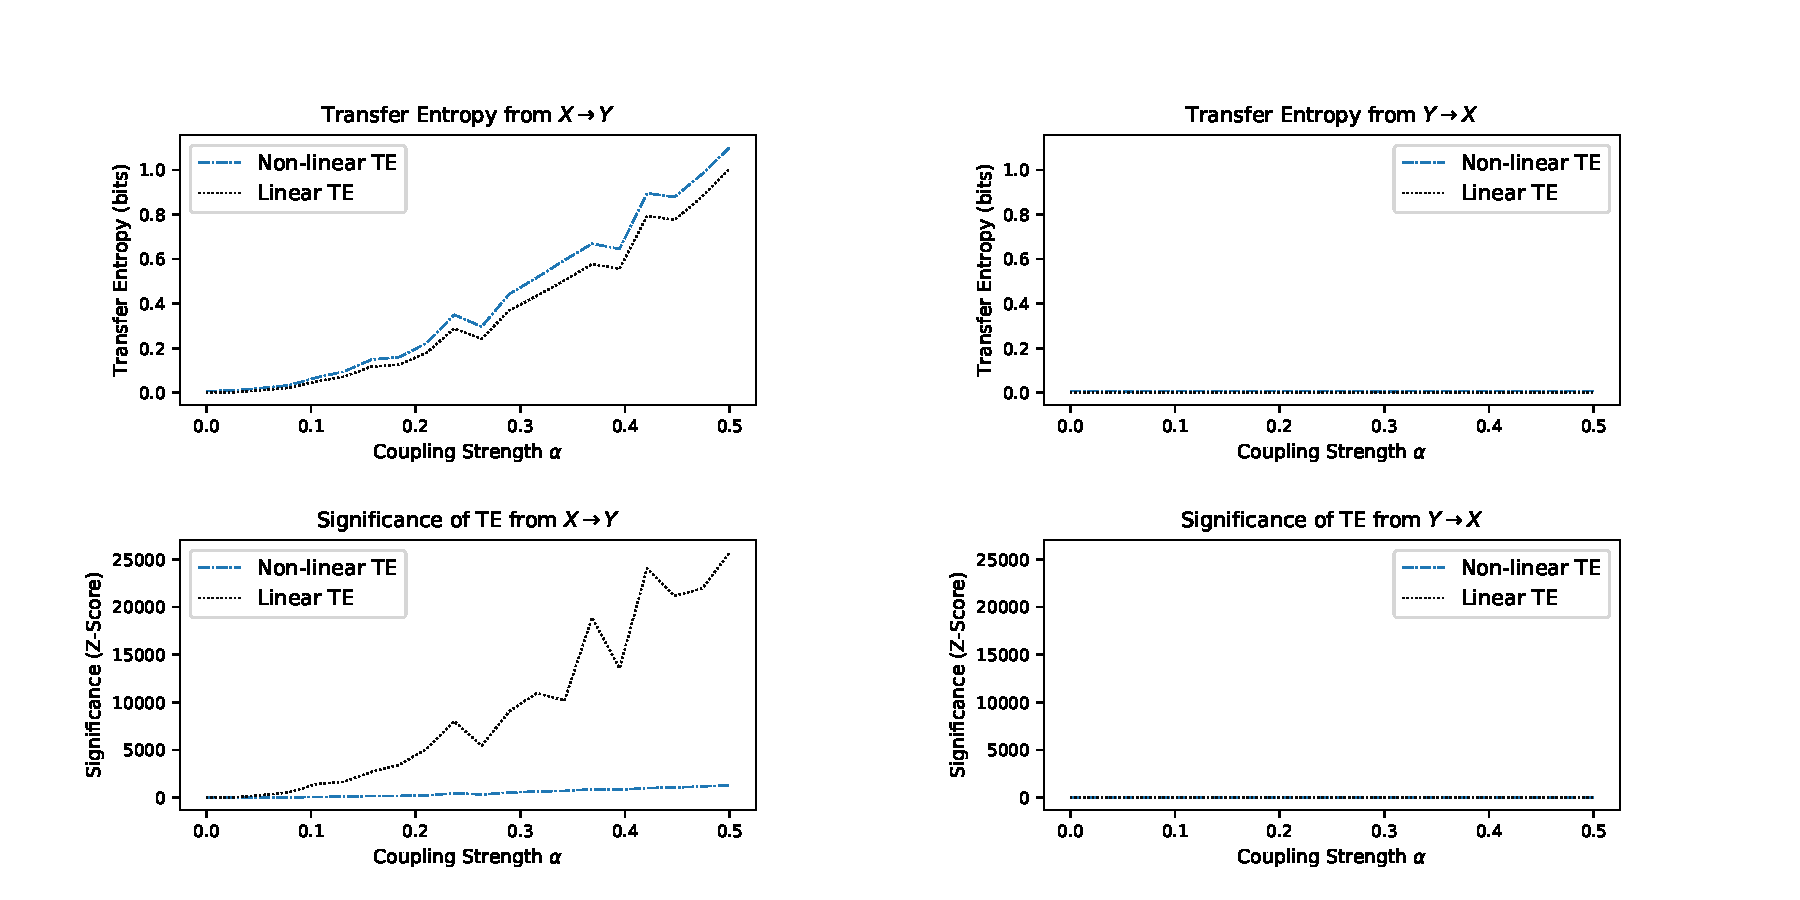
\includegraphics[width=\linewidth]{images/confirming_gbm.pdf}
    \caption{Demonstration that both linear and non-linear transfer entropy methods detect causality for linearly coupled synthetic data. The plots are calculated from the mean over 10 realisations using 15,000 data points of the synthetic random walk process from equations \ref{eq:GBM} and \ref{eq:coupled_random_walk} with $\mathbb{E} [\mu]=0.1$ and $\mathbb{E} [\mu^{\prime}]=0.1$, each with standard deviations of $0.1$, and $\mathbb{E} [\sigma]=0.025$ and $\mathbb{E} [\sigma^{\prime}]=0.025$, each with standard deviations of $0.01$.
    Non-linear transfer entropy is calculated using a quantile histogram of 6 classes per dimension. The Z-score of each result is also plotted for both methods. We observe no significant transfer entropy in the non-causal direction $Y \rightarrow X$. For the direction $X \rightarrow Y$, the Z-score of the linear technique is greater by orders of magnitude than the information-theoretic technique. However, both techniques correctly detect the linear transfer entropy, presenting largely equivalent results.}
    \label{fig:GBM_confirmation}

    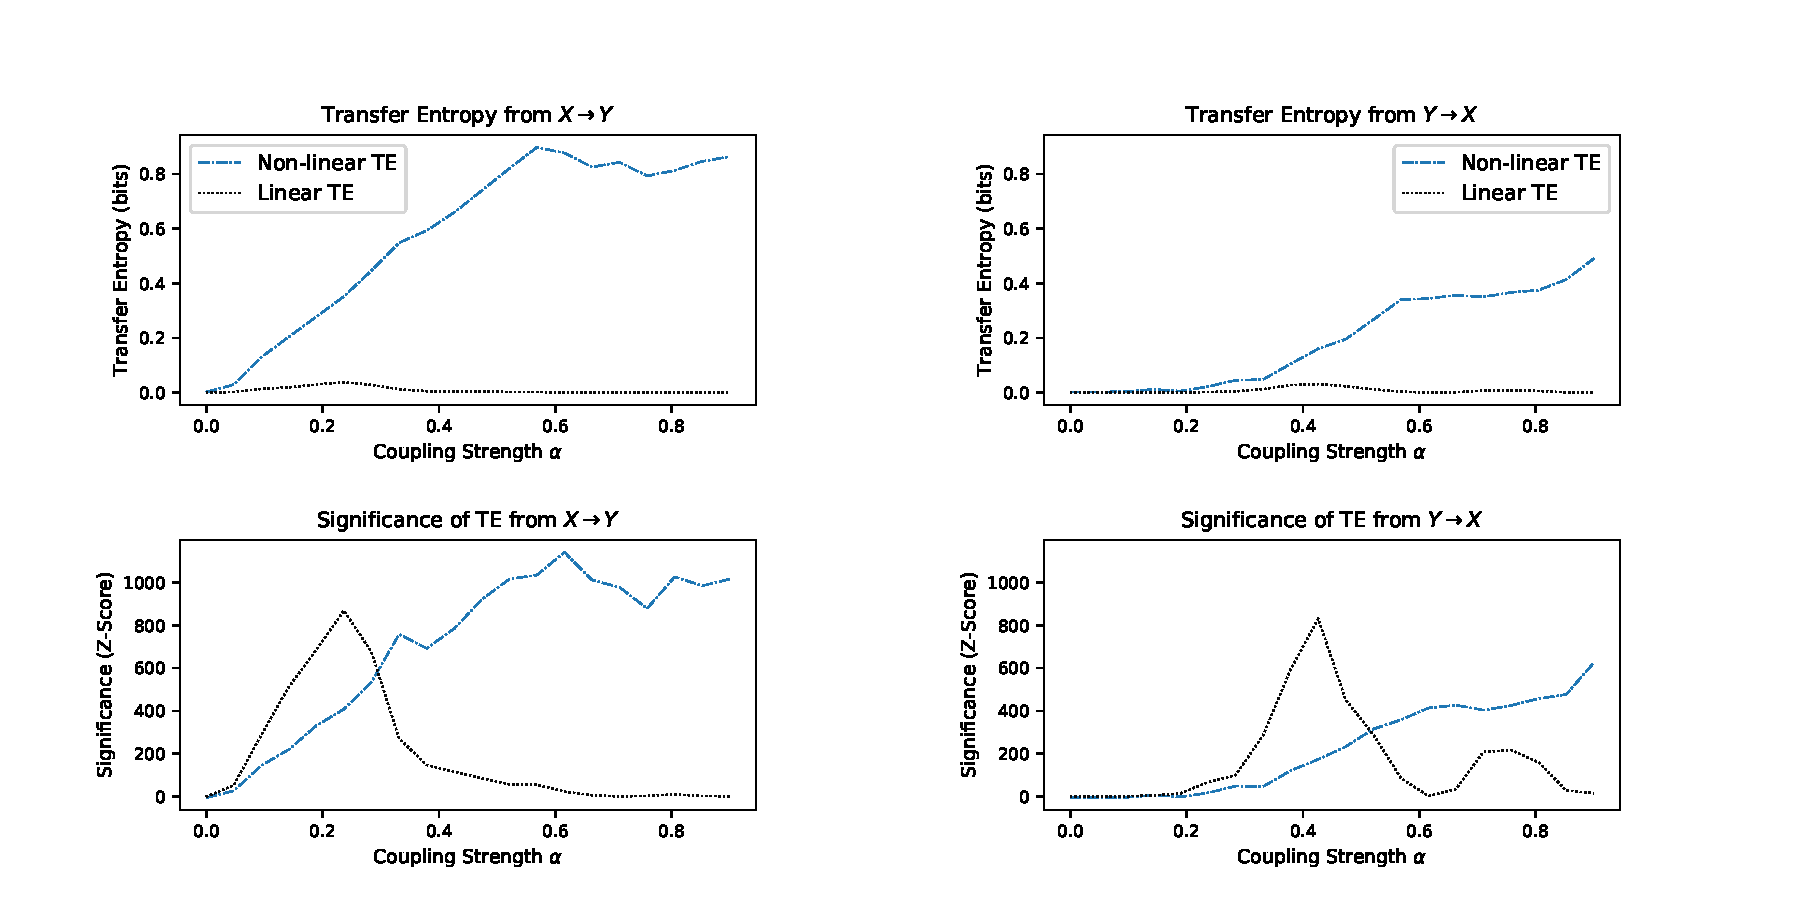
\includegraphics[width=\linewidth]{images/confirming_logmap.pdf}
    \caption{Demonstration that the non-linear causal relationship in synthetic data generated from equations \ref{eq:coupled_map} and \ref{eq:g(x)} is detected only by the non-linear method. The plots are calculated from the mean over 10 realisations over 15,000 data points of the synthetic coupled logistic map process, with $\epsilon = 0.4$. Non-linear transfer entropy is calculated using a histogram of 6 classes per dimension, partitioned using marginal equiquantisation. The Z-score for each result is also plotted for both methods. In the direction $X \rightarrow Y$, the classical approach is unable to detect the known dependency of Y on X, whilst the information-theoretic approach correctly identifies this.  We note that for $\alpha>0.2$ the information-theoretic method detects information transfer in the other direction. This is observed to increase as $\alpha$ approaches $1$, and corresponds to an expected non-linear anticipatory signal.
    }
    \label{fig:CLM_confirmation}
    %\vspace{-35pt} % Add this to rightsize the float and let it fit on a page
  \end{figure*}
  %\clearpage

  \subsection{Decay of Causal Signals with Lag Length}
  As a final validation exercise, we explore the performance of the methods in detecting signals in coupled time series when the lag of the relationship is unknown. In general, it is expected that causal links should be strongest at time-lags closest to the true signal lag, and gradually decay as the time-lag considered is increased. However, the complexity of causative relationships, particularly where any feedback exists between the time series, suggests that there could also be multi-modal causalities, operating at different lags.  

  We use the coupled GBM system defined in equations \ref{eq:GBM} and \ref{eq:coupled_random_walk} to create a coupling of a fixed lag $L=6$, and then perform both autoregressive and information-theoretic analysis to detect the transfer entropy at time-lags from $k=1$ up to $k=30$. The information-theoretic approach is applied using histograms partitioned into 6 classes per dimension, using marginal equiquantisation, and is shown to identify the specific temporal lag between driving and dependent series. The results are shown in Fig. \ref{fig:dropoff}.

  \begin{figure*}[!htb]
    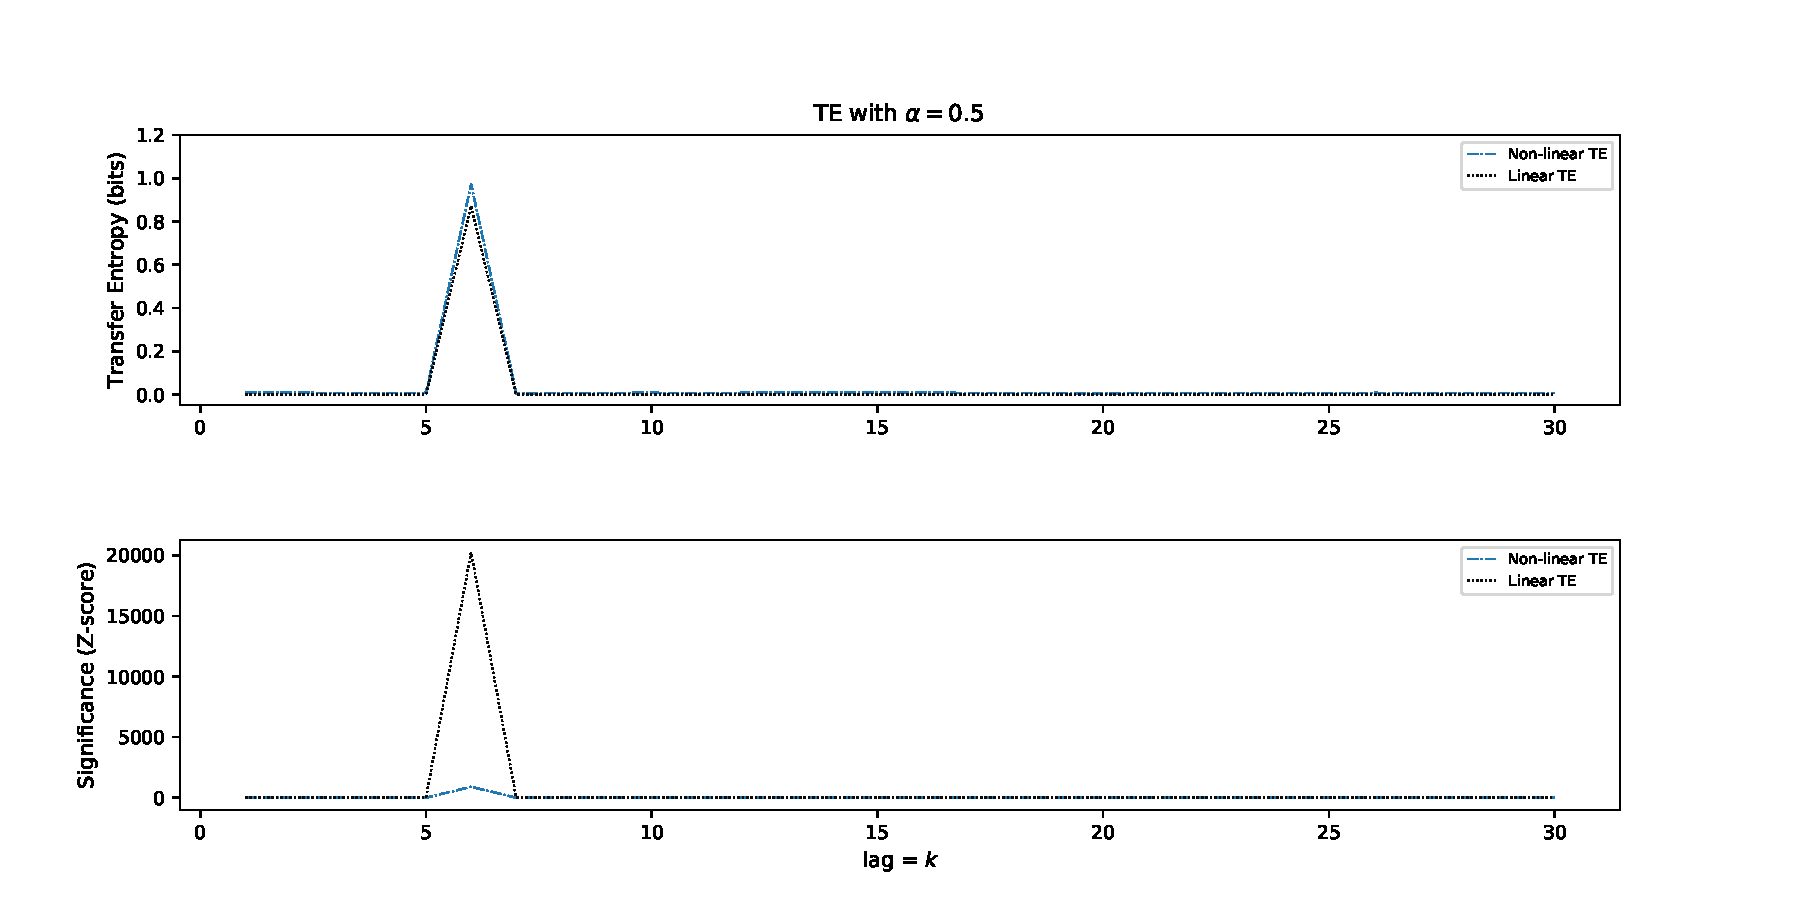
\includegraphics[width=\linewidth]{images/dropoff3.pdf}
    \caption{ Demonstration that both methods identify the true lag $L=6$  with maximal transfer entropy. Non-linear transfer entropy is calculated using a quantile-binned histogram, of 6 classes per dimension, over 15,000 points. Each result is calculated from the mean over 10 realisations. We observe zero transfer entropy in the non-causal case $\alpha = 0$, for all lags. Notably the transfer entropy of the non-causal case is non-zero using the information-theoretic technique; the Z-score for each result is also plotted for both methods, which confirms no significance is detected. In the $\alpha = 0.5$ case we observe a non-zero transfer entropy at the search length $k = L$, which corresponds to the known lag of the causal coupling $L=6$. No significant transfer entropy is observed by either technique, at all other lags. 
    }
    \label{fig:dropoff}
    
  \end{figure*}
  
  We observe the identification of the correct lag of the causal signal, which is marked by peaks at lag equal to the true lag $L=6$ of the causal relationship, and zero elsewhere. %The Z-score is much greater for the linear technique, but both methods are successful in detecting the causal coupling and the specific lead-lag period.  
  
  %Secondly, a non-zero transfer entropy observed in the decoupled case with $\alpha=0$. Notably this result is shown to be insignificant, with Z-scores roughly zero for all lags. This presents a baseline transfer entropy in this case, which might be offset against the results in the causal case $\alpha=0.1$; we note that the Effective Transfer Entropy measure could perform better in such cases, where subtracting the average zero-causality transfer entropy would give a better estimate of the true information transfer \cite{Marschinski2002}. 


%\clearpage
\section{Results with Real Data} \label{s.results}
  Having confirmed that the information-theoretic approach is able to detect both linear and non-linear causalities, we apply the technique to investigate the effect of social media sentiment on cryptocurrency prices. We also apply the linear method, and compare estimates from both techniques to establish whether linear or non-linear dynamics dominate the observed causal relationship.

  We estimate information transfer over 24-month windows, rolling forward with a stride of one month from the earliest market data available to September 2018. Each window contains $17,545$ observations of price and sentiment, sampled at hourly intervals. Price is taken as the combined close price, on the hour, over an aggregation of exchanges (see appendix \ref{a.data}). Social sentiment is estimated from NLP analysis of Twitter tweets and StockTwits during the preceding hour; we quantify this sentiment as the sum of positive messages in the previous hour. In early periods of the data, infrequently some hours have no messages; in these cases we forward-fill from the previous hour, making the assumption that sentiment does not drop to neutral in these cases. To handle non-stationarity in the data, we take the difference between the logarithms of the values at times $t$ and $t-1$. This differencing is applied to both time series. 

  The choice of timescale in aggregating raw sentiment data involves a trade-off: with too fine a timescale, there are not enough messages to estimate sentiment, but a long timescale represents a low-resolution sample which loses too much information about the underlying time series. Since cryptocurrencies are traded in real time on electronic exchanges, we hypothesise that causal signals between sentiment and price operate at sub-hourly timescales; hourly aggregation is the smallest time period available in the data, and so this aggregation of sentiment is used. 

  For the information-theoretic approach, it is observed that performing the analysis with histograms of equal-width bins gives different results depending on the number of bins selected. Specifically, partitioning the axes of the sample space into odd-numbers of bins produces no significant result over this data, suggesting the information is captured mostly from the middle peak of the distribution. However, we note that the use of quantile binning avoids this issue, finding both odd-numbered and even-numbered bin counts to provide similar results, suggesting a key benefit in using quantile bins for the calculation of transfer entropy. Accordingly, in this analysis we partition the sample space into quantile bins, using six classes per dimension, having validated this choice in Section \ref{s.validation}. The histogram bins for the non-linear approach are calculated once, using the full data set for each currency, and then they are applied across all windows. In selecting an appropriate partition, further bias is inevitably introduced. By calculating appropriate bins for each window, the results cannot be directly compared between windows. However, the growth in message volumes over time means that selecting bins sized to capture the full spread of values would also introduce a bias, since such bins are more suited to the later months than the earlier months. Since the granularity of the histogram partition also impacts the transfer entropy value, we perform significance tests over each window independently, calculating the Z-scores and comparing these across windows and currencies.  We report the windows with greatest significance using a time-lag of $k=1\operatorname{hour}$. Performing the analysis using longer time-lags shows weaker causal signals over this data. This provides evidence in support of the hypothesis that the true causal dynamics operate at sub-hourly timescales.

  Plots showing the information transfer for the four cryptocurrencies investigated are reported in Fig. \ref{fig:BTC_TE}, Fig. \ref{fig:LTC_TE}, Fig. \ref{fig:XRP_TE} and Fig. \ref{fig:ETH_TE}. Z-scores for each result are also presented; for comparison across figures, Z-score axes  use the same scale.
  
  For BTC, in Fig. \ref{fig:BTC_TE}, we detect a strong causative signal, of roughly similar scale in both directions of sentiment to BTC price and in the reverse direction. Analysis of the Z-scores confirms the significance in both directions, with the net information transfer greater in the direction of price to sentiment, with mean net transfer entropy of $-0.0016$ bits.
  
  LTC, in Fig. \ref{fig:LTC_TE}, shows a similar pattern to BTC, although in this case the predominant direction of information transfer is reversed, with mean net transfer entropy of $0.0039$ bits. The Z-scores show the significance of sentiment to price is consistently greater than in the reverse direction, and also stronger than the other currencies. In addition, there is notably a large linear component to the information transfer, which is unique to LTC. 

  XRP, in Fig. \ref{fig:XRP_TE}, shows a clear non-linear causality from sentiment to price, with a significant but smaller causal relationship also in the opposite direction. The mean net transfer entropy is measured for this period as $0.0022$ bits. The signal is more significant from sentiment to price, and especially in the periods ending in 2018. 
  
  ETH, in Fig. \ref{fig:ETH_TE}, shows an interesting and unique behaviour. In particular, there appears to be, initially, a significant signal which collapses in the windows ending around January 2018. The information transfer at its initial peak is greater from price to sentiment, however over the whole period the effect is more bidirectional, with mean net transfer entropy of zero. This suggests a slight phase change, with sentiment driving price after the collapse of the signal, although no net significance is observed after this point in either direction. This strongly indicates another driving mechanism, the effect of which first becomes present around January 2016 (due to 24-month windows). This effect is likely to be associated with the rapid price movements at the time.  %\cite{Ethereum} 
  
  \begin{figure*}[!htbp]
    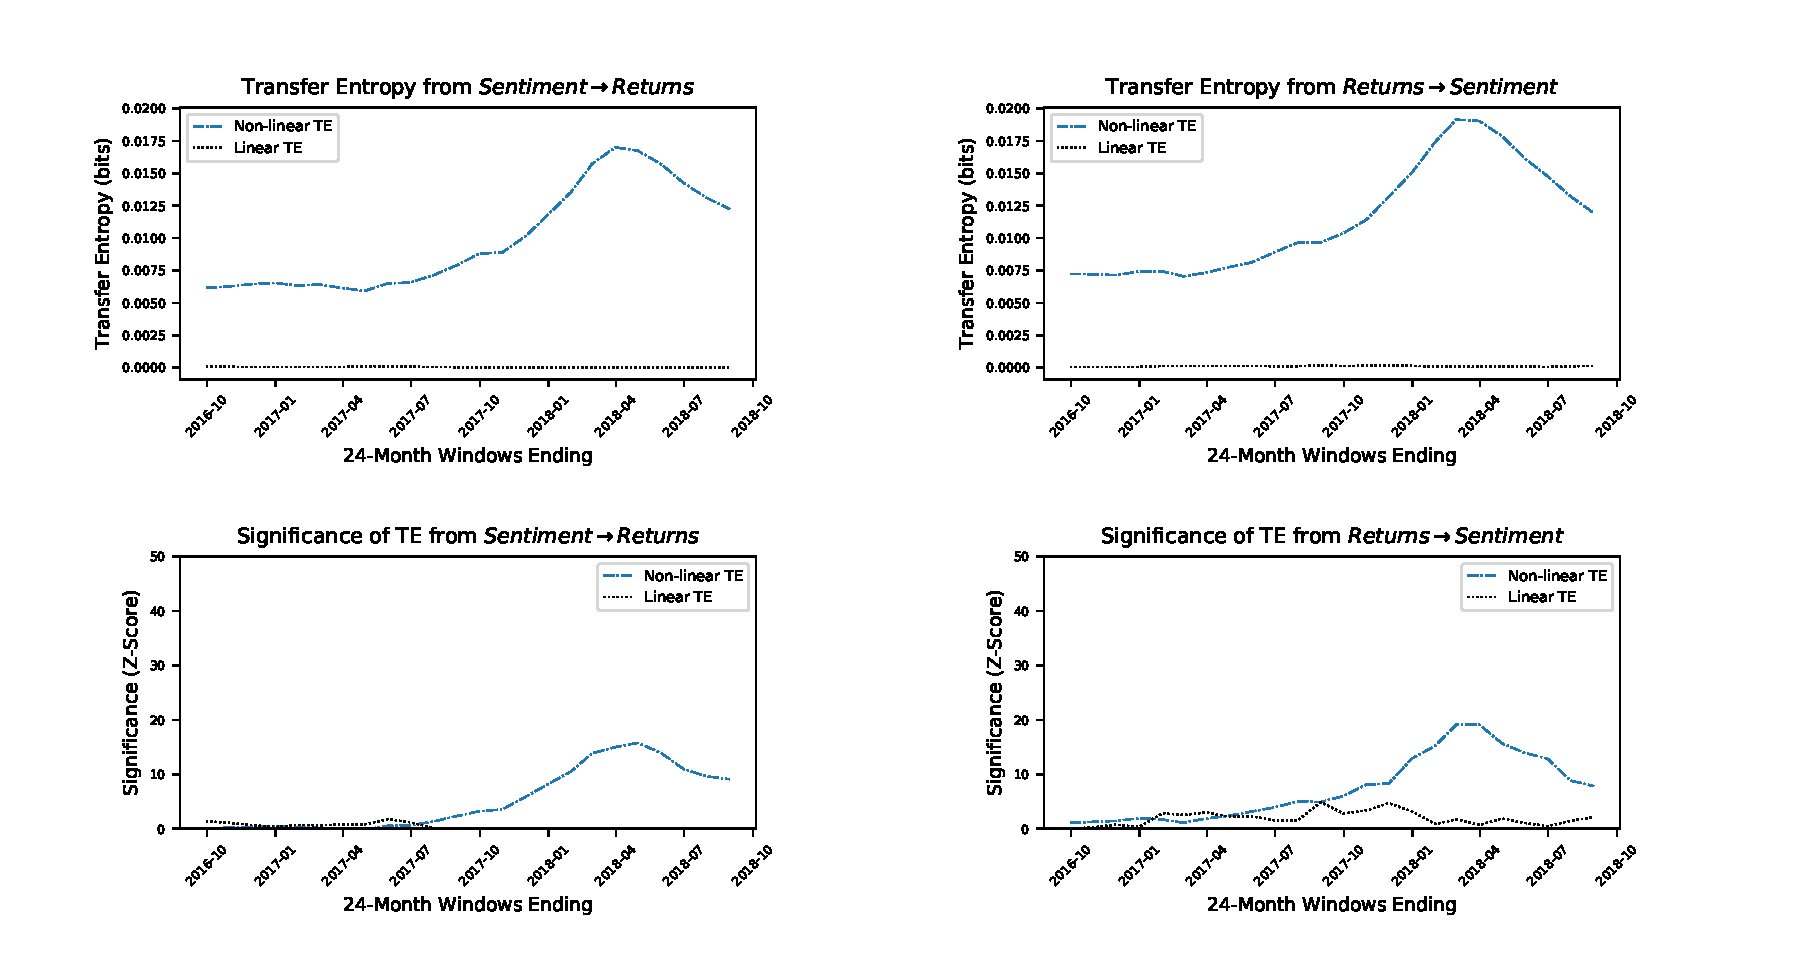
\includegraphics[width=\linewidth]{images/BTC.pdf}
    \caption{Evidence that BTC sentiment and price are causally coupled in both directions in a non-linear way. Non-linear TE is calculated by multidimensional histograms with 6 quantile bins per dimension. Z-scores, calculated over 100 shuffles, show a high level of significance, especially during 2017 and 2018, in both directions, with the peak significance $Z=21.3$ observed in the direction of price to sentiment in the 24-month window ending February 2018.}
    \label{fig:BTC_TE}
  
    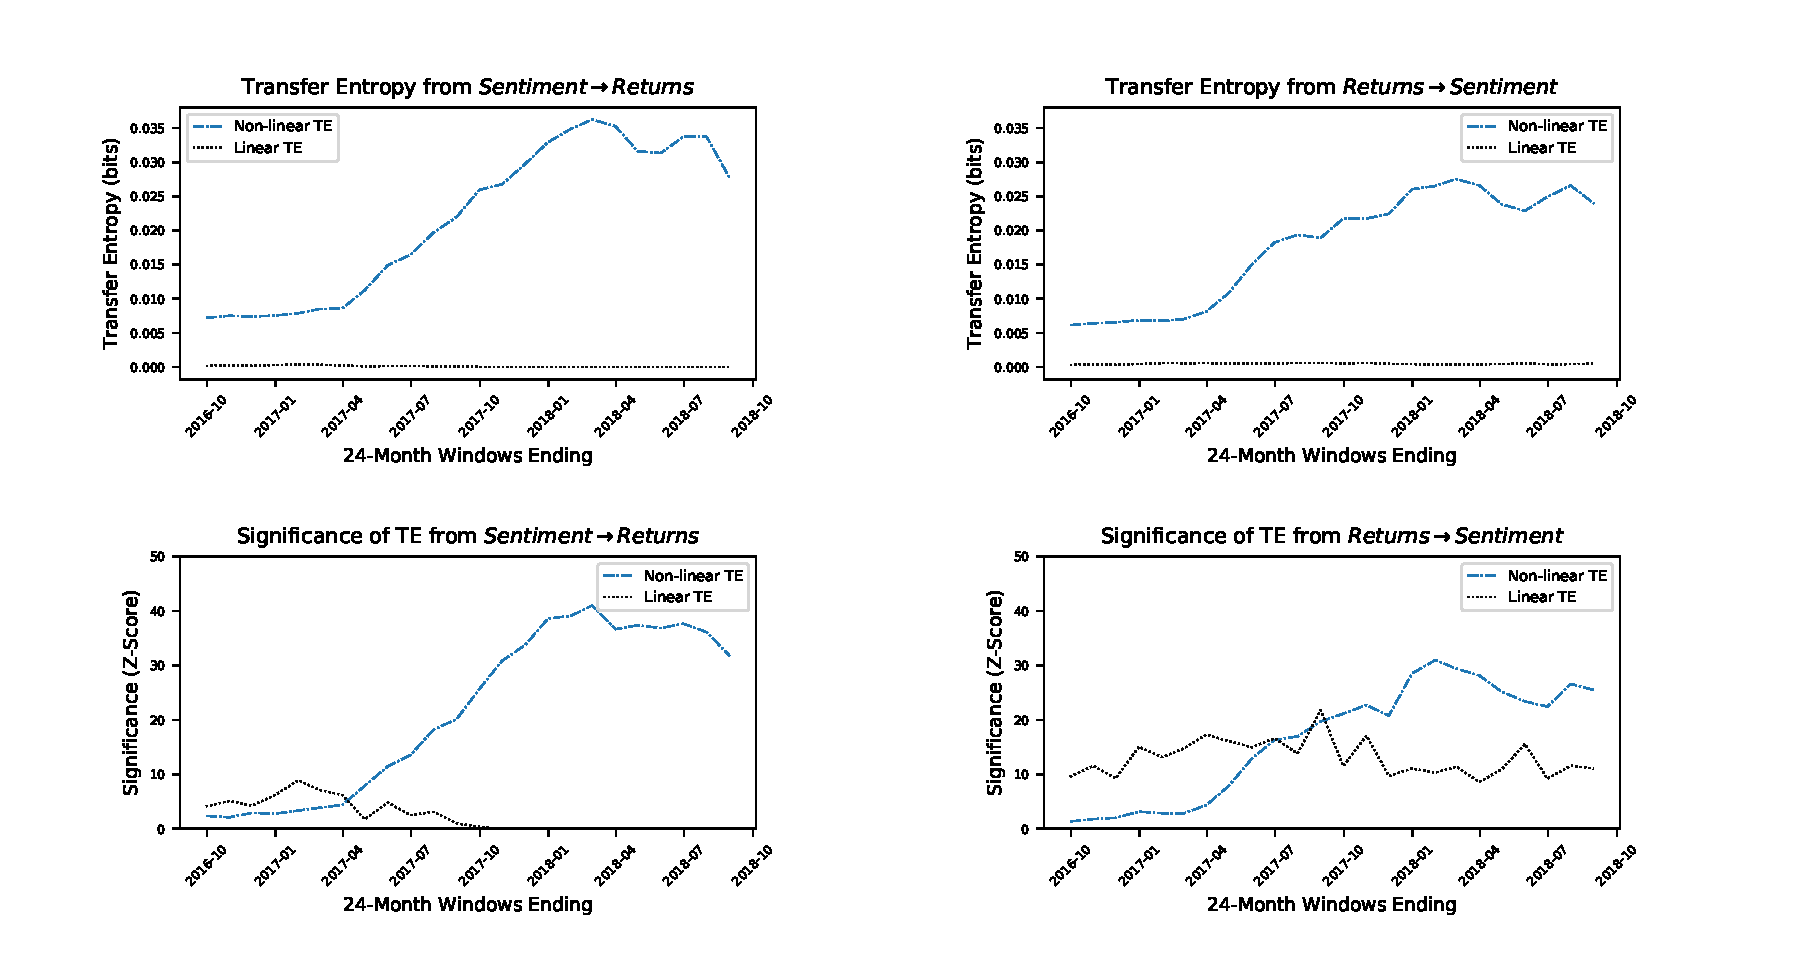
\includegraphics[width=\linewidth]{images/LTC.pdf} 
    \caption{Evidence that LTC price and sentiment are causally coupled in both directions in a non-linear way, with sentiment having a larger influence on price than the other way round. Non-linear TE is calculated by multidimensional histograms with 6 quantile bins per dimension. Z-scores, calculated over 100 shuffles, show a significant signal in both directions, with the net information transfer generally operating in the direction of sentiment to price. Peak significance of $Z=42.8$ is observed from sentiment to price in the 24-month window ending February 2018.}
    \label{fig:LTC_TE}
    \vspace{-4pt}
  \end{figure*}

  \begin{figure*}[!htbp]
    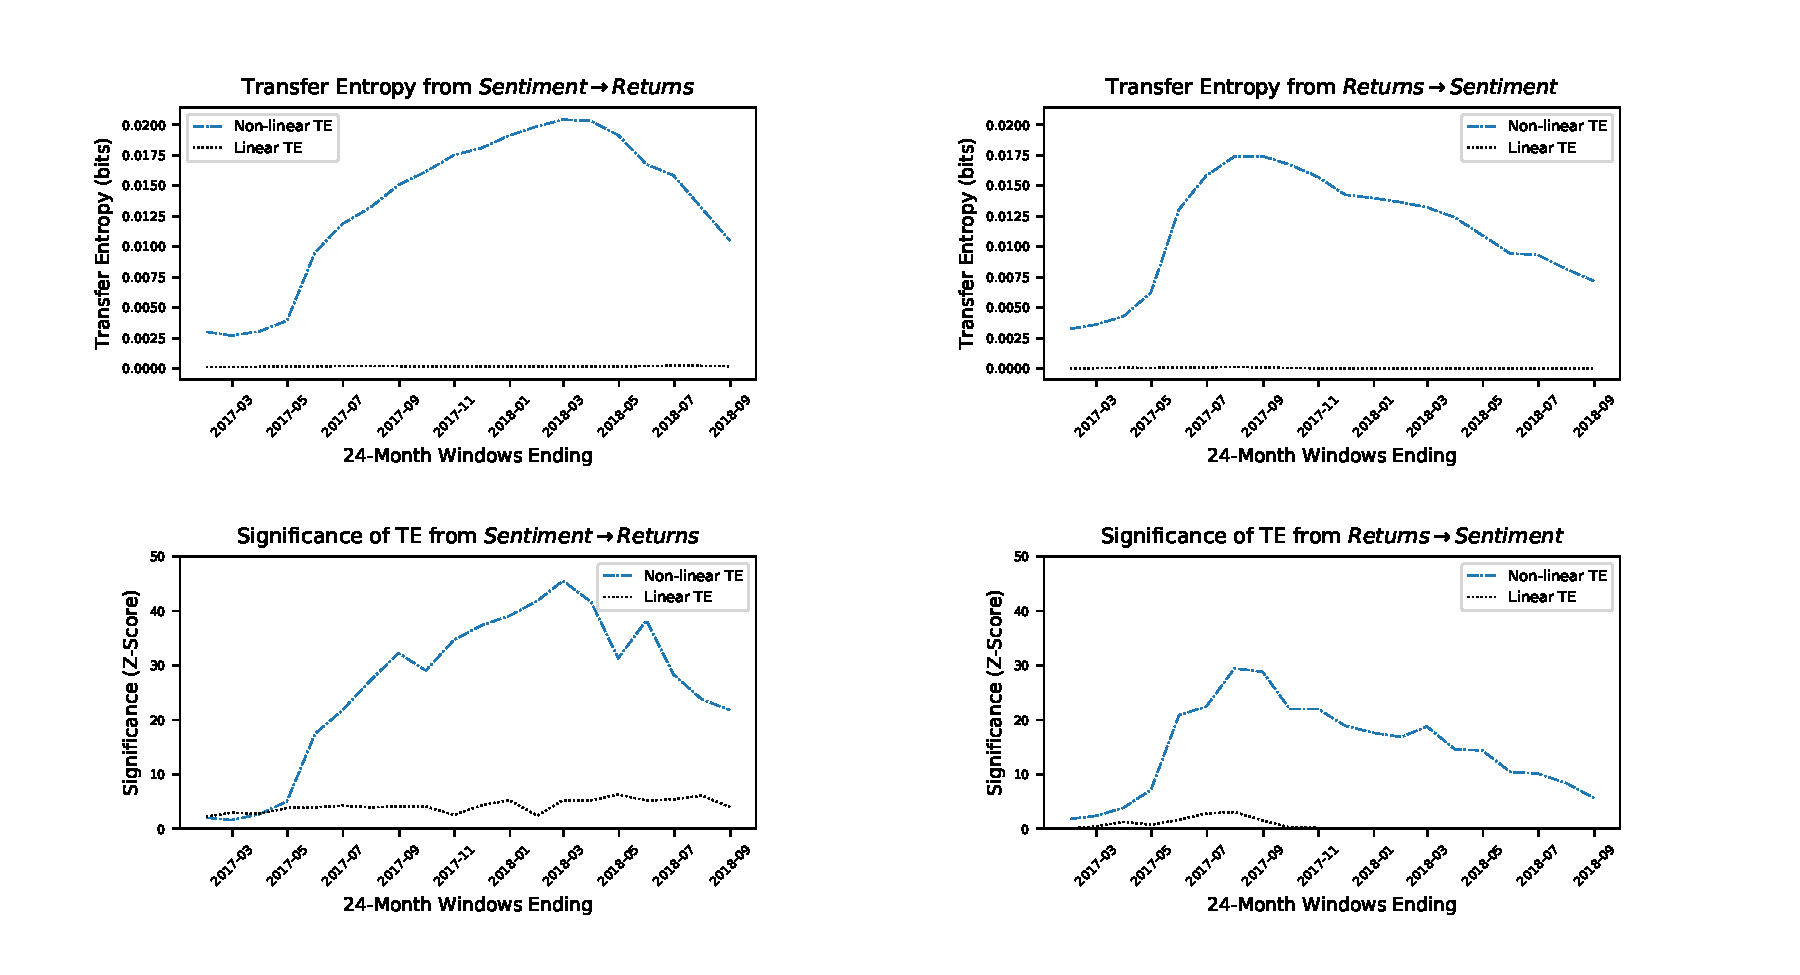
\includegraphics[width=\linewidth]{images/XRP.pdf}
    \caption{Evidence that XRP price and sentiment are causally coupled in both directions in a non-linear way, with the prevailing direction of information transfer flowing from sentiment to price in the first period, and from price to sentiment in the second. Non-linear TE is calculated by multidimensional histograms with 6 quantile bins per dimension. Z-scores, calculated over 100 shuffles, show a small but clear significant signal, in both directions, which decays rapidly towards January 2018 and does not recover afterward. Peak significance of $Z=41.9$ is observed from sentiment to price in the 24-month window ending January 2018.}
    \label{fig:XRP_TE}

    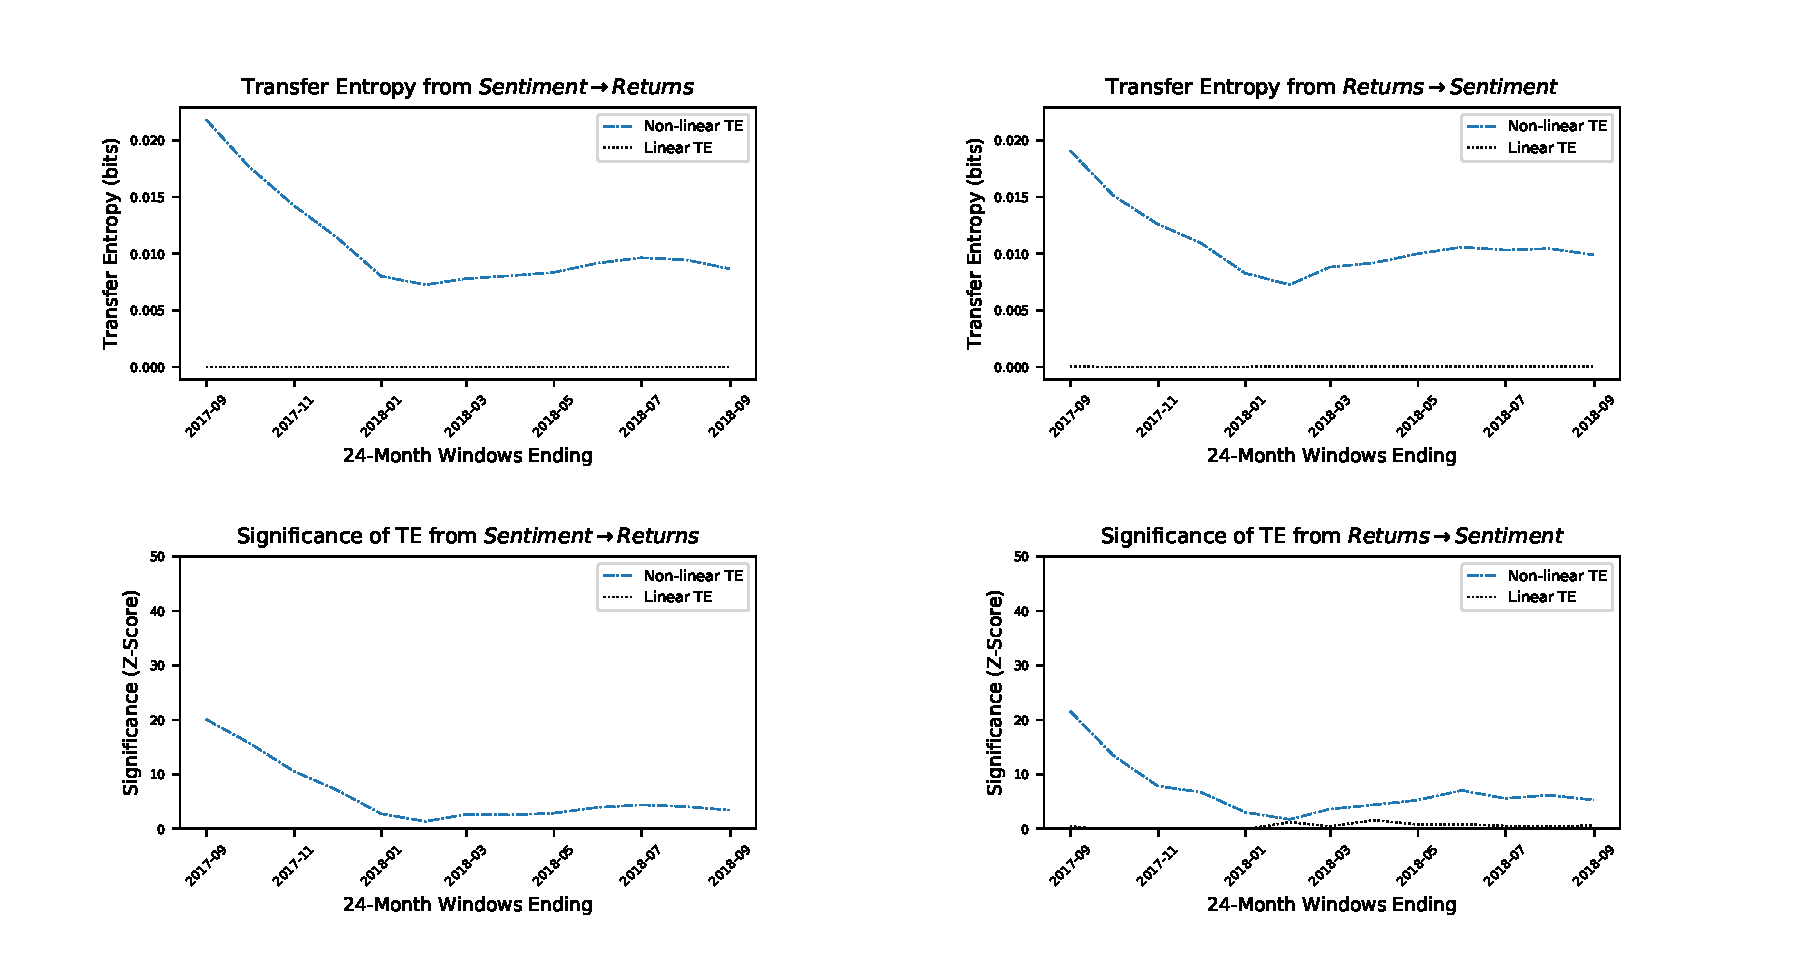
\includegraphics[width=\linewidth]{images/ETH.pdf} 
    \caption{Evidence that ETH price and sentiment are causally coupled in both directions in a non-linear way. Overall this coupling is of lower significance compared to the other currencies investigated. Non-linear TE is calculated by multidimensional histograms with 6 quantile bins per dimension. Z-scores, calculated over 100 shuffles, indicate initial significance for windows ending before 2018, followed by low significance after the collapse in signal strength, which must therefore begin around January 2016. Peak significance is observed in the first window of the study, with $Z=20.6$ in the direction of sentiment to price, and $Z=19.9$ in the direction of price to sentiment.     
  }
  \label{fig:ETH_TE}
  \vspace{-34pt}
  \end{figure*}
  
 
\clearpage
\section{Conclusion} \label{s.conclusions}

Information-theoretic and autoregressive techniques were developed and validated on coupled random walks and chaotic logistic maps, confirming the ability of both techniques to detect linear information transfer, and of the information-theoretic technique to detect non-linear information transfer. Following validation, the techniques were applied to historical data describing social media sentiment and cryptocurrency prices to detect information transfer between sentiment and price movements. 

The information-theoretic investigation detected a significant non-linear causal relationship in BTC, LTC and XRP, over multiple timescales and in both directions of sentiment to price and price to sentiment. The effect was strongest and most consistent for LTC and XRP, and in both cases the net information transfer was in the direction of sentiment to price. ETH and BTC were observed to show significant net information transfer in the direction price to sentiment, although separate dynamics were observed in ETH which see a collpase in significance. Given the hypothesis that low barriers to entry and unsophisticated investor speculation are key drivers for price movements, and that BTC and ETH represent the most widely known and traded cryptocurrencies, the fact that causality is detected most clearly for these currencies corresponds to expectations.

The significance tests confirm the existence of causally-coupled relationships, though the strength of these relationships are challenging to accurately quantify from the data, especially for the purposes of comparison between different time series, and between the linear and non-linear results over the same data. However, the significance values themselves offer the possibility of quantifying the strength of causality, which may be used as a proxy when using transfer entropy as a tool for detecting statistical causality. With this work we demonstrate that the dynamics of the causative relationship is non-linear, as the autoregressive technique was able to detect only small or zero causality in either direction, for any of the currencies. The mean Z-scores of results observed by linear and information-theoretic methods are presented for each currency in Table {\color{blue}4}. Our results show that histograms of marginal equiquantisation, in concert with permutation tests, can be used in practice to detect nonlinear information transfer between time series, even where classical statistical techniques fail. Let us point out that there is a risk of assuming ergodicity in the results; we have shown that the level of causation varies historically within the sample time period, and there is no evidence that the observed causal relationships will continue unchanged. 


%\clearpage


\section{Appendix}

 \subsection{Estimate of mutual information and transfer entropy from relative frequencies}
 In order to compute the mutual information or the transfer entropy, we must estimate entropies from Eq.\ref{eq:entropy}.
 The histogram approach discretises the continuous sample space by partitioning it into bins that - in general - are not assumed to be of equal size, and so transforms the integral into a sum.
  \begin{eqnarray}
    \label{eq:entropyDiscrere}
    H(X) = - \int_{-\infty}^{+\infty}  {  p(x) \log{  p(x)}  } dx \simeq - \sum_{x_k}  \hat p(x_k) \log\left({ \hat p(x_k)}\right) v(x_k)\;.
  \end{eqnarray}
Where $\hat p(x_k)$ is the estimate of the probability density function $p(x)$ computed for the bin $x_k$ that contains the observation $x$.
The quantity $v(x_k)$ is the proportion of the support of the probability density function which is occupied by the bin. This generalises to multiple dimensions.
The estimate of the probability density function $\hat p(x_k)$ can be computed from the number of observations $n(x_k)$ that fall in each bin via
    \begin{eqnarray}
    \label{eq:pdfDiscrere}
 \hat p(x_k) = \frac{n(x_k)}{N v(x_k)}\;,
  \end{eqnarray}
where $N=\sum_{x_k} n(x_k)$ is the total number of observations. 
The entropy estimation is therefore:
  \begin{eqnarray}
    \label{eq:entropyDiscrere1}
    H(X) \simeq - \sum_{x_k}   \frac{n(x_k)}{N } \log\left({  \frac{n(x_k)}{N v(x_k)} }\right) \;.
  \end{eqnarray}
This quantity depends on the relative volumes of the bins, and hence do the estimates for $H(Y)$ and $H(X,Y)$ also require these to be calculated. However, in the mutual information $I(X;Y) = H(X)+H(Y)-H(X,Y)$ the terms containing the volumes cancel, and its expression turns out to be dependent only on the relative frequencies:
  \begin{eqnarray}
    \label{eq:mutualnfoDiscrere}
  I(X;Y) \! \simeq \!
 \! \!\sum_{x_k,y_j} \!\!\frac{n(x_k,y_j)}{N } \log\left({  \frac{n(x_k,y_j)}{N} }\right)
   -\! \sum_{x_k}      \! \frac{n(x_k)}{N } \log\left({  \frac{n(x_k)}{N} }\right) 
  - \!\sum_{y_j}        \!\frac{n(j_j)}{N } \log\left({  \frac{n(y_j)}{N} }\right) .
  \end{eqnarray}
  The same applies to the transfer entropy. 
  This is a remarkable simplification of the computation of these quantities, which shows how they can be estimated from histograms simply in terms of the relative frequencies, for any kind of binning partition.
 
  \subsection{Source Code}
    All analysis for this paper was performed using a Python package (PyCausality) created by the lead author. This is maintained on the author's public GitHub profile, which can be found at \url{https://github.com/ZacKeskin/PyCausality}. For the latest release this can be simply installed via PyPi using pip. 

    Synthetic data as presented in this paper can be generated using the functions made available in the package test utils, in Time\_Series\_Generate.py. This contains code to produce coupled time series either of the chaotic logistic map or of geometric Brownian motion. To replicate the validation experiments in Section \ref{s.validation}, time series should be generated with parameters $T=1$, $N=15,000$ for the coupled random walk, and with parameters $T=10$, $N=15,000$ and $\epsilon=0.4$ for the coupled logistic map. 

    Ongoing maintenance and pre-release development of the package will be made available through this repository, and contributors may fork code and submit pull requests to develop this further.


  \subsection{Data} \label{a.data}

  The social sentiment data was provided courtesy of PsychSignal, and may be made available pending request to the authors. The data takes the form of the number of positive messages and the number of negative messages, publicly shared on either Twitter or StockTwits, associated each hour with the cryptocurrencies in question. The association is detected via the use of a `hashtag' (or `cashtag') which takes the form of \#BTC or \#Bitcoin (for example) on twitter, or \$BTC on StockTwits.  For inclusion in the dataset, the message must contain one of the tags described in Table {\color{blue}1}.  
  
  Price data is the hourly close in USD, obtained via CryptoCompare's public API. This provides a combined average over multiple exchanges, where prices are available. For further details, the documentation is available at \url{https://min-api.cryptocompare.com/}

  \begin{table*}[!htb]
    \label{t.table1}
    \caption{\label{tab:table1} Hashtags used to map social media messages to specific cryptocurrencies.}
    
      \begin{tabular}{cccc}
        Curency & Tag & Curency & Tag        \\ [0.5ex] 
        \hline 
        Bitcoin & BTC &  Litecoin & LTC.X    \\
        Bitcoin & BCOIN & Litecoin & LTCUSD  \\
        Bitcoin & BTC.X & Ripple & XRP.X     \\
        Bitcoin & BTCEUR & Ripple & XRPBTC   \\
        Bitcoin & BTCGBP & Ripple & XRPUSD   \\
        Bitcoin & BTCUSD & Ethereum & ETH    \\
        Bitcoin & GBTC & Ethereum & ETH.X    \\\
        Bitcoin & SGDBTC & Ethereum & ETHUSD \\
      \end{tabular}
    
    \end{table*}

  
  \subsection{Tables} \label{a.tables}

  Analysis was undertaken to validate the performance of linear and non-linear techniques over multiple parameter values for sample size and signal strength. Table {\color{blue}2} contains the Z-scores of transfer entropy calculations using marginal equiquantisation, for coupled random walks of increasing coupling strength and sample size. 
  
  Table {\color{blue}3} contains results quantifying the net information transfer across windows of the study for each cryptocurrency. Net information transfer is calculated as $ \operatorname{TE}^{(1)}_{X \rightarrow Y} - \operatorname{TE}^{(1)}_{Y \rightarrow X} $, and is given in units of bits.

  
  \begin{table*}[!htb]
    \label{t.table2}
    \caption{ Z-scores of transfer entropy from $X$ to $Y$, for coupled GBM system described in Section \ref{s.validation}. Calculated using the information-theoretic technique for increasing sample size $n$ and coupling strength $\alpha$}
    
      \begin{tabular}{lrrrr}

    n       &         0 &       0.1 &       0.3 &       0.5 \\
    \hline 
    500.0    & -0.0 &     0.8 &     6.5 &     9.8 \\
    1000.0   &  0.1 &    10.7 &    13.5 &    42.1 \\
    2500.0   &  0.2 &     6.5 &    69.9 &    57.1 \\
    10000.0  & -0.2 &    57.6 &   272.5 &   225.3 \\
    100000.0 & -0.1 &  1339.7 &  2387.3 &  2254.8 \\

    \end{tabular}
    
  \end{table*}

  \begin{table*}[!htb]
    \label{t.table3}
    \caption{ Net information transfer statistics in units of bits determined over all windows of the study for each cryptocurrency. Mean values show that in time, more information was transfered from sentiment to price for LTC and XRP, with more information transfer in the direction of price to sentiment for BTC and ETH. It should be noted that mean due to the overlapping strides of the windows, periods during the middle of the sample are weighted more heavily; however the figures appropriately present the relative direction of information transfer over the 48-month period of the study, so are presented for the sake of comparison. Significance scores are presented in Table {\color{blue}4}.}

    
    \begin{tabular}{lrrr}
     {} &    Mean &  10th Percentile &  90th Percentile \\
     \hline 
     BTC & -0.0016 &          -0.0032 &          -0.0005 \\
     LTC &  0.0039 &           0.0004 &           0.0086 \\
     XRP &  0.0022 &          -0.0036 &           0.0074 \\
     ETH & -0.0001 &          -0.0014 &           0.0023 \\
    \end{tabular}
  
  \end{table*}


  \begin{table*}[!htb]
    \label{t.table4}
    \caption{Table of average Z-scores across all windows of observation for each currency. We observe nonlinear values generally an order of magnitude greater than the linear values, with the exception of LTC for which we see relatively large linear components. However the nonlinear transfer entropy remains considerably larger than the linear values even for LTC.}
    
    \begin{tabular}{lrrrr}
      {} & {} & (Price $\rightarrow$ Sentiment) & {} & (Sentiment $\rightarrow$ Price)  \\
      {} & Linear  &  NonLinear  &  Linear  &  Nonlinear  \\
      \hline 
      % BTC &     0.1 &     2.0 &        5.1 &        7.6 \\
      % LTC &     2.2 &    11.8 &       22.4 &       17.3 \\
      % XRP &     4.1 &     0.4 &       24.1 &       14.4 \\
      % ETH &    -0.6 &     0.5 &        6.5 &        6.8 \\
      BTC &     0.1 &       5.1 &       2.0 &        7.6 \\
      LTC &     2.2 &      22.4 &      11.8 &       17.3 \\
      XRP &     4.1 &      24.1 &       0.4 &       14.4 \\
      ETH &    -0.6 &       6.5 &       0.5 &        6.8 \\
      \end{tabular}
    
  \end{table*}


  \pagebreak

%%%%%%%%%% Acknowledgements etc. %%%%%%%%%%%%%%

  \vskip10pc

  \dataccess{Social sentiment Data was provided courtesy of PsychSignal, and may be made available pending request to the authors.}

  \funding{TA acknowledges support from ESRC (ES/K002309/1),  EPSRC (EP/P031730/1) and EC (H2020-ICT-2018-2 Fin-Tech 825215).}
  
  \ack{The authors acknowledge Th\'arsis Souza in advising on the method of testing for linear Granger causality, with thanks along with Yuqing Long, whose data collation and wrangling was a great help. Finally, a great debt of thanks is to PsychSignal for providing their market sentiment data for this academic study.}

%%%%%%%%%% Bibliography  %%%%%%%%%%%%%%

\vskip2pc

\bibliographystyle{RS} %%%% .BST file

\bibliography{references} %%%%% .Bib file

\end{document}
